\documentclass[main.tex]{subfiles}
\begin{document}

\section{Sheet 10}

\subsection{Allowed Kerr orbits}

\subsubsection{\(\Omega \) inequality}

The condition we want to impose is \(u^{\mu } g_{\mu \nu } u^{\nu } = -1\). Explicitly, since the four-velocity is  \(u^{\mu } = u^{t} \qty(1, 0, 0, \Omega )\), this means that 
%
\begin{align}
  (u^{t})^2 \qty(g_{00} + 2 g_{03} \Omega + g_{33} \Omega^2 ) = -1
\,.
\end{align}

We can work up to a positive multiplicative factor, at the price of weakening our equality to an equality: since \((u^{t})^2 > 0\), we can also write 
%
\begin{align}
  g_{00} + 2 g_{03} \Omega + g_{33} \Omega^2 < 0
\,,
\end{align}
%
and since many of the terms contain divisions by \(\rho^2\) we can also multiply by \(\rho^2>0\) which will not change the sign; also we flip the sign of the inequality since we have more negative terms than positive ones (both of these really are for consistency with the assignment):
%
\begin{align}
 - \rho^2 \qty(g_{00} + 2 g_{03} \Omega + g_{33} \Omega^2 ) > 0 
\,.
\end{align}

Now we can substitute in the Kerr metric components (which we will not need to remember by heart): 
%
\begin{align}
  \rho^2 - 2GMr 
  + \qty(4 GMra \sin^2\theta ) \Omega 
  - \qty(\rho^2 (r^2 + a^2 ) + 2GMra^2 \sin^2\theta ) \sin^2(\theta)  \Omega^2 > 0
\,,
\end{align}
%
so we can read off the values of the coefficients \(c_{n}\) as everything multiplying \(\Omega^{n}\), for \(n = 0, 1, 2\): 
%
\begin{subequations}
\begin{align}
    c_0 &= \rho^2 - 2GM r   \\
    c_1 &= 4 GMra \sin^2\theta   \\
    c_2 &= - \qty(\rho^2 (r^2 + a^2 ) + 2GMra^2 \sin^2\theta ) \sin^2(\theta)
\,.
\end{align}
\end{subequations}

\subsubsection{Ergosphere characterization}

The ergosphere, as was discussed during the lectures, is defined as the region in which there are no timelike worldlines which are stationary with respects to the spatial coordinates, that is to say, with velocity parallel to the vector \((1, \vec{0})\).
This is equivalent to saying that the metric component \(g_{00} > 0\), which corresponds to a region which extends beyond the horizon, and is shaped like an ellipsoid for low \(a/GM\) and like a donut without the hole for high \(a/ GM\).\footnote{See the python folder (or, possibly, the notes later) for visualizations of this.}

Now, \(c_0 = - \rho^2 g_{00} \), so \(c_0 < 0\) is equivalent to \(g_{00} > 0\). 
The characterization of the ergoregion is a special case of the prolem we are discussing now, where we fix \(\Omega = 0\).

\subsubsection{Inequality discriminant}

We start by writing everything out the pieces separately: 
%
\begin{align}
  \frac{c_1^2}{4} = 
  \frac{16}{4} \qty(GMar \sin^2\theta)^2 
\,,
\end{align}
%
while
%
\begin{align}
\begin{split}
    - c_0 c_2  = 
    + \sin^2\theta  \big(&\rho^{4} \qty(r^2+a^2) + \rho^2 2 GMa^2 r \sin^2\theta +\\
    &- 2GMr \rho^2 (r^2+a^2) - 4 \qty(GMra \sin \theta )^2\big)
    \,,
\end{split}
\end{align}
%
so we can see that the last term in \(- c_0 c_2 \) precisely cancels \(c_1 ^2 /4\): we are then left with 
%
\begin{align}
  \frac{c_1^2}{4}-c_0 c_2 &= \sin^2 \theta \qty(\rho^{4} \qty(r^2+a^2) + \rho^2 2 GMa^2 r \sin^2\theta 
  - 2GMr \rho^2 (r^2+a^2))  \\
  &= \rho^{4} \sin^2\theta \qty(\qty(r^2+a^2) - 2GMr \qty(\frac{r^2+a^2 - a^2 \sin^2\theta }{\rho^2}))  \\
  &= \rho^{4} \sin^2\theta \qty(r^2+a^2-2GMr)
\,,
\end{align}
%
where in the last step we used the fact that \(r^2+a^2 \qty(1 - \sin^2\theta ) = r^2+a^2 \cos^2\theta = \rho^2\). 

\subsubsection{Allowed angular velocities}

We have a second degree polynomial inequality, and the quadratic coefficient \(c_2 \) is negative: therefore as \(\abs{\Omega } \rightarrow \infty \) the parabola in \(\Omega \) goes to \(- \infty \), so if there are any solutions to the inequality they are an interval between the two solutions of the equation \(\sum c_{n} \Omega^{n} = 0\).\footnote{This is just the way I like to remember which solutions to select, but in the end it's just a quadratic inequality, solve it however you like.}

These are given by the quadratic formula 
%
\begin{align}
  \Omega_{+, -} = \frac{- c_1/2 \pm \sqrt{c_1^2/4- c_0 c_2  }}{c_2 }
\,,
\end{align}
%
which gives: 
%
\begin{align}
\Omega_{-,+} &= \frac{-2GMra \sin^2\theta \pm \sqrt{\rho^4 \sin^{2}\theta \qty(r^2+a^2-2GMr)}}{- \sin^2\theta \qty(\rho^2(r^2+a^2)+2GMra^2 \sin^2\theta )}  \\
&= \frac{2GMra \mp \rho^2 \sqrt{ \qty(r^2+a^2-2GMr) / \sin^2 \theta }}{\rho^2(r^2+a^2)+2GMra^2 \sin^2\theta }
\,,
\end{align}
%
which I do not think can be simplified further. 
Do note that we did not use the hypothesis of being in the ergosphere: the bounds for the angular velocity are general, it's just that in the ergosphere they preclude \(\Omega = 0\). 

Do these solutions actually exist? They do if \(r^2+a^2-2GMr = \Delta >0\) (the \(\Delta \) from the definition of the Kerr geometry). Recall that this \(\Delta \) is positive outside the outer horizon and inside the inner horizon: in the region between the outer horizon and the ergosphere the solutions are well defined. 
This region is precisely the ergoregion. 

\subsubsection{Corotation necessity}

We want to show that in the ergoregion, which is defined by \(\rho^2 < 2GMr\) and \(\Delta >0\), we have that \(\Omega > 0 \) for any solution for our inequality. This is equivalent to saying that the lower of the two solutions for the equality (let us say the lower one is \(\Omega_-\)) must be \(>0 \) in this case. The denominator is always positive, so we can discard it. Then we want to show that 
%
\begin{align}
2GMra - \rho^2 \sqrt{(r^2+a^2-2GMr) / \sin^2\theta }  > 0
\,,
\end{align}
%
which can be rephrased as 
%
\begin{align}
\abs{\sin(\theta )} 2GMra > \rho^2 \sqrt{r^2+a^2-2GMr}
\,.
\end{align}

In adimensional units \(A = a/GM\), \(R = r / GM\) and \(P^2 = R^2+A^2 \cos^2\theta \) this becomes 
%
\begin{align}
4 \sin^2\theta R^2A^2 > P^4 \qty(R^2-2R + A^2)
\,,
\end{align}
%
while our ergoregion is defined by: 
%
\begin{align}
R^2- 2R + A^2 > 0 > R^2 - 2R + A^2 \cos^2\theta 
\,.
\end{align}

Only the \(R>1\) region is accessible without crossing an horizon: then we can solve the equations and find 
%
\begin{align}
 \sqrt{1 - A^2} < R-1 < \sqrt{1 - A^2 \cos^2\theta }
\,.
\end{align}
%

\todo[inline]{AAAAA can't figure out how to prove it}

\subsubsection{Single allowed speed}

If \(\Delta = 0\), then the two solutions to the quadratic equation collapse: only one speed is allowed, and it is equal to 
%
\begin{align}
\Omega = \frac{2GMra}{\rho^2 \qty(r^2+a^2) + 2GMr a^2 \sin^2\theta }
\,,
\end{align}
%
which we can simplify using \(r^2+a^2 = 2GMr\) (which is  precisely \(\Delta = 0\)): 
%
\begin{align}
\Omega = \frac{2GMra}{2GMr \qty( \rho^2 + a^2 \sin^2 \theta )} = \frac{a}{r^2 + a^2 \qty(\cos^2\theta +\sin^2\theta )} = \frac{a}{2GMr}
\,,
\end{align}
%
where the radius is precisely that of the (outer) horizon, the greatest solution  to \(\Delta = 0\). 

\subsubsection{Extreme Kerr equatorial orbit}

We set \(a = GM\) and \(\theta  = 0\). Then we have \(\rho^2= r^2\), \(\cos \theta = 0\) and \(\sin \theta =1\), so
%
\begin{align}
\Omega_{1, 2} &= \frac{2 (GM)^2 r \mp r^2\sqrt{r^2 + (GM)^2 - 2GMr}}{r^2 \qty(r^2 +(GM)^2) + 2 (GM)^3 r}  \\
&= \frac{2 (GM)^2 \mp r \abs{r - GM}}{r^3+(GM)^2r + 2 (GM)^3} \\
O_{1,2}&= \frac{2 \mp R (R-1)}{R^3+R + 2}
\,,
\end{align}
%
where the absolute value is redundant since we are working at \(r > GM\).
We introduced adimensionalized variables \(O = GM \Omega \) and \(R = r/GM\), which make the expressions way simpler. Using these is equivalent to setting \(GM = 1\). 

The upper bound is given by the solution with the plus sign: 
%
\begin{align}
O_{+} = \frac{R^2 - R + 2}{R^3+ R  + 2} = \frac{1}{1 + R}
\,;
\end{align}
%
to check that this is indeed the case one can simply multiply the polynomials together. 
How might one guess or calculate this? If we want to divide the denominator by the numerator, we could use the algorithm of polynomial division, but there is a faster way. By inspection of the exponents we might guess that the result is a first degree polynomial in \(R\), and looking at the coefficients one can see that both the coefficient of \(R\) and the constant in this first order polynomial must be 1. This ansatz can then be checked by multiplication. Reinserting \(GM\), we get 
%
\begin{align}
\Omega_{+} = \frac{1}{GM + r}
\,.
\end{align}
%

For the lower bound we get: 
%
\begin{align}
O_{- } = \frac{- R^2 + R + 2 }{R^3 + R + 2} 
= - \frac{(R+1) (R-2)}{(R+1) (R^2-R+2)} 
= \frac{2-R}{R^2-R+2}
\,,
\end{align}
%
where we used the decomposition of the denominator we had derived in the last paragraph, and the regular quadratic decomposition for the numerator. Reinserting \(GM\), this is 
%
\begin{align}
\Omega_{-} = \frac{2GM-r}{r^2- rGM +2 (GM)^2}
\,,
\end{align}
%
which I find to be simpler than the equivalent decomposition proposed in the assignment, which is 
%
\begin{align}
\frac{1}{GM} \qty(1 - \frac{r^2}{2(GM)^2-GMr +r^2}) 
&= \frac{1}{GM} \qty(\frac{2(GM)^2-GMr +r^2 - r^2}{2(GM)^2-GMr +r^2})  \\
&= \frac{2GM - r}{2(GM)^2-GMr +r^2}
\,.
\end{align}
%
\begin{figure}[ht]
  \centering
  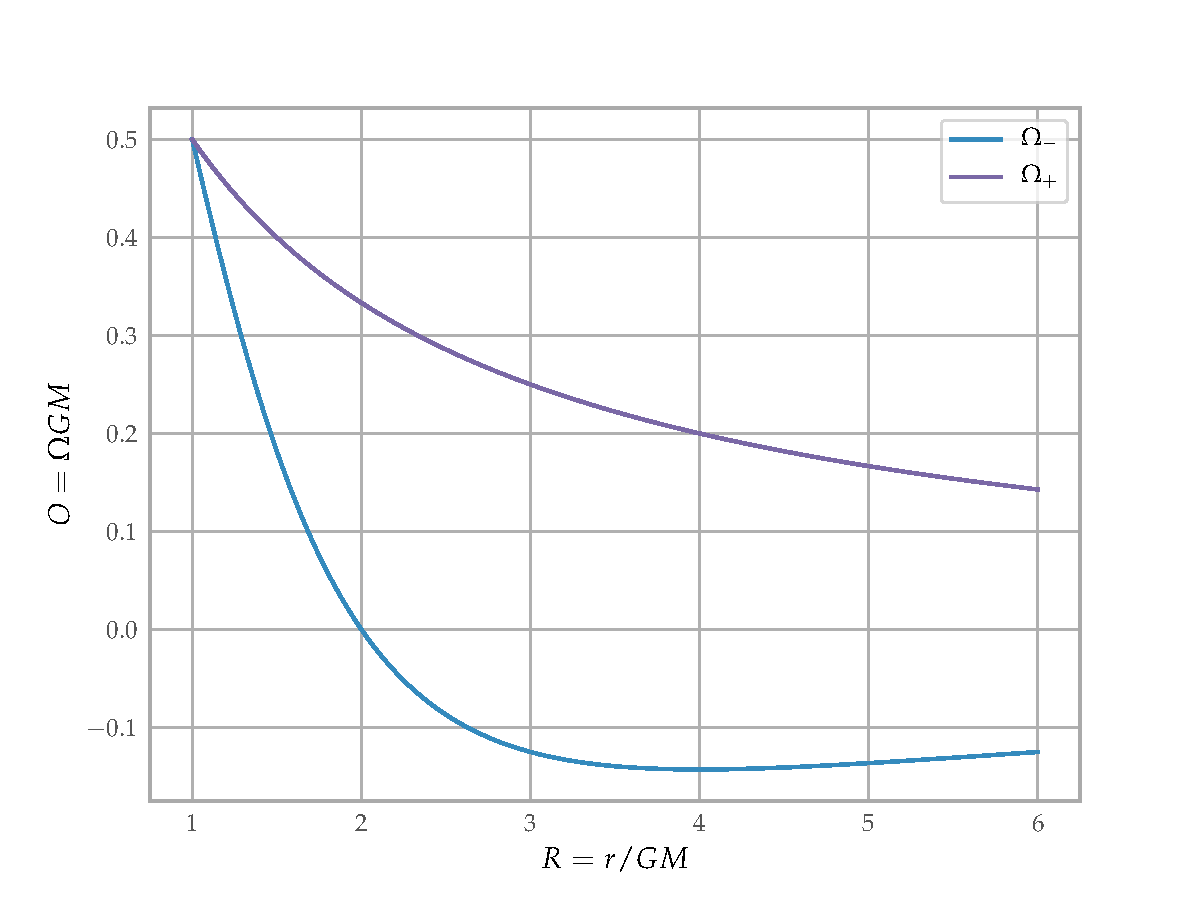
\includegraphics[width=\textwidth]{figures/allowed_velocities.pdf}
  \caption{Allowed angular velocities.}
  \label{fig:allowed-velocities}
\end{figure}

A plot of these limiting velocities is shown in figure \ref{fig:allowed-velocities}: we can see that for \(1<R<2\) (that is, inside the ergoregion) we must have a positive \(\Omega \).

It is interesting to note that both \(\Omega_{\pm}\) tend to 0 as \(R \rightarrow \infty \): this makes sense since the \emph{tangential} velocity which corresponds to \(\Omega \) is \(r \Omega \), which approaches \(\pm 1\) for \(\Omega_{\pm}\), as we'd expect. 

\subsection{Natural units}

Let us denote the numeric value of the time in seconds by \(\mathtt{t}\), so that \(t = \mathtt{t} \SI{}{s}\). It will be given by 
%
\begin{align}
\mathtt{t} = \frac{1}{\SI{}{GeV s}} \times \hbar^{\alpha } c^{\beta } = \frac{\SI{}{J}}{\SI{}{GeV}} \times \frac{1}{\SI{}{Js}} \times \hbar^{\alpha } c^{\beta }  
\,,
\end{align}
%
where we inserted some generic powers of \(\hbar\) and \(c\), to be determined through dimensional analysis.
We should write a system of linear equations for the exponents, but since the units of the reduced Planck constants are \SI{}{Js} we can already say that the solution will be \(\alpha = 1\), \(\beta =0\). 
So, the value will be 
%
\begin{align}
\mathtt{t}  = \frac{\SI{}{J}}{\SI{}{GeV}} \times \frac{\hbar}{\SI{}{Js}} = \SI{6.58e-25}{}
\,.
\end{align}

We can use the exact same procedure to get the value of the length in meters, as defined by \(L = \mathtt{L} \SI{}{m}\). We find \(\alpha = \beta = 1\): 
%
\begin{align}
\mathtt{L} = \frac{\SI{}{J}}{\SI{}{GeV}} 
\times \frac{\hbar}{\SI{}{Js}} \times \frac{c }{\SI{}{m s^{-1}}} = \num{1.97e-16}
\,.
\end{align}

If everything we have is in SI units, we can drop them so the computations become quite fast: up to SI units we have \(t  = \hbar / (\num{e9}e) \) and \(L = \hbar c / (\num{e9} e)\).

The number of seconds in a year is approximately given by \(3600 \times 24 \times 365.25 = 31557600 \approx \pi \times \num{e7}\).

\subsection{Friedmann equations derivation}

This was done during lectures, I will copy it here sometime. 

\end{document}
